%%%%%%%%%%%%%%%%%%%%%%%%%%%%%%%%%%%%%%%%%%%%%%%%%%%%%%%%%%%%%%%%%%%%%%%%%%%
%%%                                                                     %%%
%%%   LaTeX template voor het verslag van P&O: Computerwetenschappen.   %%%
%%%                                                                     %%%
%%%   Opties:                                                           %%%
%%%     tt      Tussentijdsverslag                                      %%%
%%%     eind    Eindverslag                                             %%%
%%%                                                                     %%%
%%%   7 februari 2014                                                   %%%
%%%   Versie 1.2                                                        %%%
%%%                                                                     %%%
%%%%%%%%%%%%%%%%%%%%%%%%%%%%%%%%%%%%%%%%%%%%%%%%%%%%%%%%%%%%%%%%%%%%%%%%%%%

\documentclass[tt]{penoverslag}

%%% PACKAGES %%%
\usepackage{graphicx}
\usepackage{amsmath}
\usepackage{wasysym}
\usepackage{float}
\usepackage{wrapfig}
\setlength\parindent{0pt}

\begin{document}

% == TITELPAGINA == %
\team{Indigo} % teamkleur
\members{
        Wander Bavin\\
        Vince Goossens\\
        Dimitri Jonckers\\
        Sunil Tandan\\
        Wout Vekemans} % teamleden
\maketitlepage


% == SAMENVATTING == %
\begin{abstract}
\noindent
Dit rapport documenteert onze analyse en oplossing van het volgende probleem : de constructie en operatie van een zeppelin in wedstrijdverband. Navigatie gebeurt op basis van een op voorhand gekend grondplan dat wordt ingeladen in de software. De positie van de zeppelin wordt bepaald door een algoritme gebaseerd op beeldherkenning. Via het rooster dient de zeppelin sneller dan een andere zeppelin naar een bepaalde positie te vliegen, en een andere, nog onbekende opdracht uitvoeren. Beide zeppelins wisselen informatie uit met elkaar en met hun sturende pc via een server gebaseerd op RabbitMQ. Een GUI dient de toestand van het speelveld met beide zeppelins te visualiseren. Al deze functionaliteiten worden ge\"{i}mplementeerd in Java.
\end{abstract}


% == INHOUDSOPGAVE == %
\tableofcontents\newpage


% == INLEIDING == %
\section{Inleiding}
Dit tweede deel van de bachelorproef draait nog steeds rond het aansturen van een zeppelin op basis van een Raspberry Pi. 

\paragraph{Fysisch ontwerp}
~\\
De zeppelin bestaat uit een houten frame waaraan 2 heliumballonnen ($\diameter$90 cm) vastgemaakt zijn. Aan het frame zijn een camera en een afstandssensor vastgemaakt, die beiden naar beneden gericht zijn. Zowel de camera als de afstandssensor zijn verbonden met een Raspberry Pi die in het frame zit ingebed. Het geheel bevat drie propellers: twee voor horizontale bewegingen en \'{e}\'{e}n voor verticale bewegingen.


\paragraph{Software ontwerp}
~\\
De software die inwendig op de Pi draait en op de client-pc voor image processing en weergave van de GUI is geschreven in Java. De communicatie tussen de zeppelin en de client gebeurt via een server. (Zie figuur \ref{schema}). \\

TODO !!!! schema figuur
\begin{figure}[ht!]
\centering
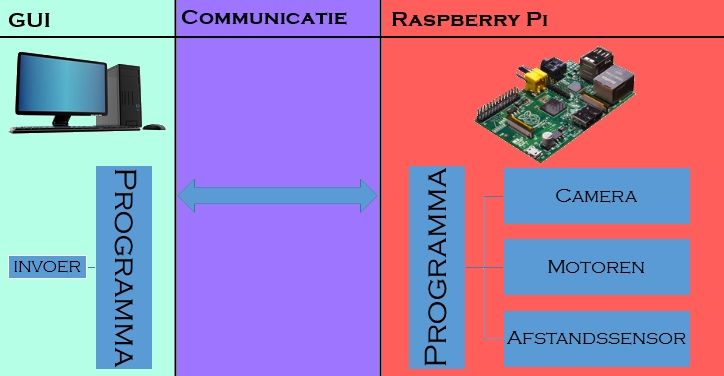
\includegraphics[height=55mm]{Schema.jpg}
\caption{Architectuur}
\label{schema}
\end{figure}

% == Beschrijving materiaal en bouw zeppelin == %
\section{Beschrijving materiaal en bouw zeppelin}
De zeppelin bestaat uit een frame waaraan alle onderdelen zijn vastgemaakt. Hierop worden onder andere de 3 propellers bevestigd. Twee hiervan dienen om in het horizontale vlak te bewegen. Ze zijn met haakse draairichting op het frame gemonteerd. De derde propeller, om de zeppelin te laten stijgen, is naar beneden gericht. De propellers kunnen op volle kracht of door middel van pwm\footnote{en.wikipedia.org/wiki/Pulse-width\_modulation} worden aangestuurd (in 2 richtingen). Met deze techniek is het mogelijk om naast de richting ook de kracht van de motor in te stellen. De onderste propeller wordt aangestuurd door de wired pwm op het motorbordje, terwijl voor de horizontaal gerichte propellers gebruik wordt gemaakt van SoftPWM\footnote{https://github.com/Pi4J/pi4j/blob/master/pi4j-core/src/main/java/com/pi4j/wiringpi/SoftPwm.java}. ~\\

\begin{figure}[h!]
\centering
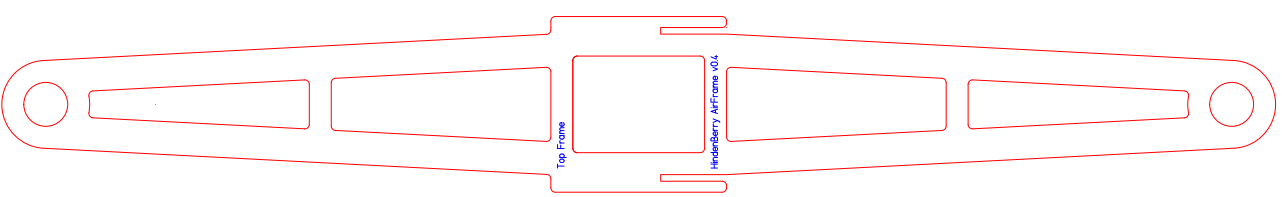
\includegraphics[scale=0.3]{upperFrame.png}
\label{frame}
\end{figure}

\begin{figure}[h!]
\centering
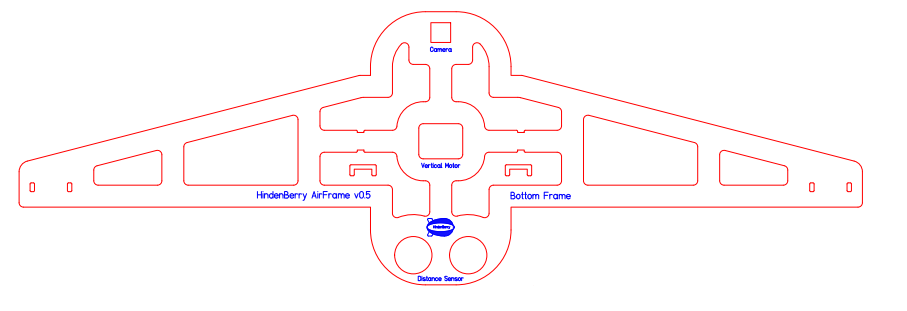
\includegraphics[scale=0.3]{lowerFrame.png}
\caption{Blueprint van het frame}
\label{frame}
\end{figure}

Om het geheel in de lucht te houden, zitten er 2 heliumballonnen ($\diameter$90 cm) vast aan de bovenkant van het frame. Deze hebben initieel een lift van 268 gr per stuk, maar dit vermindert wanneer de ballonnen doorheen de weken volume verliezen. \\

De zeppelin wordt aangestuurd door een Raspberry Pi model A. Deze heeft volgende specificaties:
\begin{itemize}
\item \emph{Processor:} 700MHz ARM
\item \emph{Geheugen:} 256MB
\item \emph{Poorten:} 1 USB 2.0, HDMI, audio out, RCA video
\item \emph{Voeding:} Micro USB
\item GPIO-pinnen om de hardware aan te sturen
\end{itemize}

In de Raspberry Pi zit een SD-kaart van 4 GB. Hierop staat Raspbian, het standaard besturingssysteem van de Raspberry Pi. Er is nog voldoende ruimte over om onze eigen programma's als jar-file op de Pi te zetten. \\

Verder zijn er nog 2 devices waarvan de zeppelin gebruik maakt:
\begin{itemize}
\item \emph{De camera} laat toe foto's te nemen met een maximum resolutie van 5 MP. Deze wordt in deze opdracht vooral gebruikt voor het bepalen van de positie van de zeppelin. Hiervoor neemt hij foto's van de patronen op de grond die gematcht worden met het gekende grondplan. Daarnaast kan de camera video's maken met resoluties tot 1080p.
\item \emph{De afstandssensor} kan worden gebruikt om met ultrasone trillingen de afstand te meten tussen de zeppelin en de grond of muur. De sensor heeft een bereik van 2-400 cm. Onze afstandssensor is vooral gebruikt voor het aansturen van het hoogteregelend PID-algoritme.  \\
\end{itemize}


{\Large NEED FOR AN UPDATED FIGURE!!! }\\
%\begin{figure}[ht!]
%\centering
%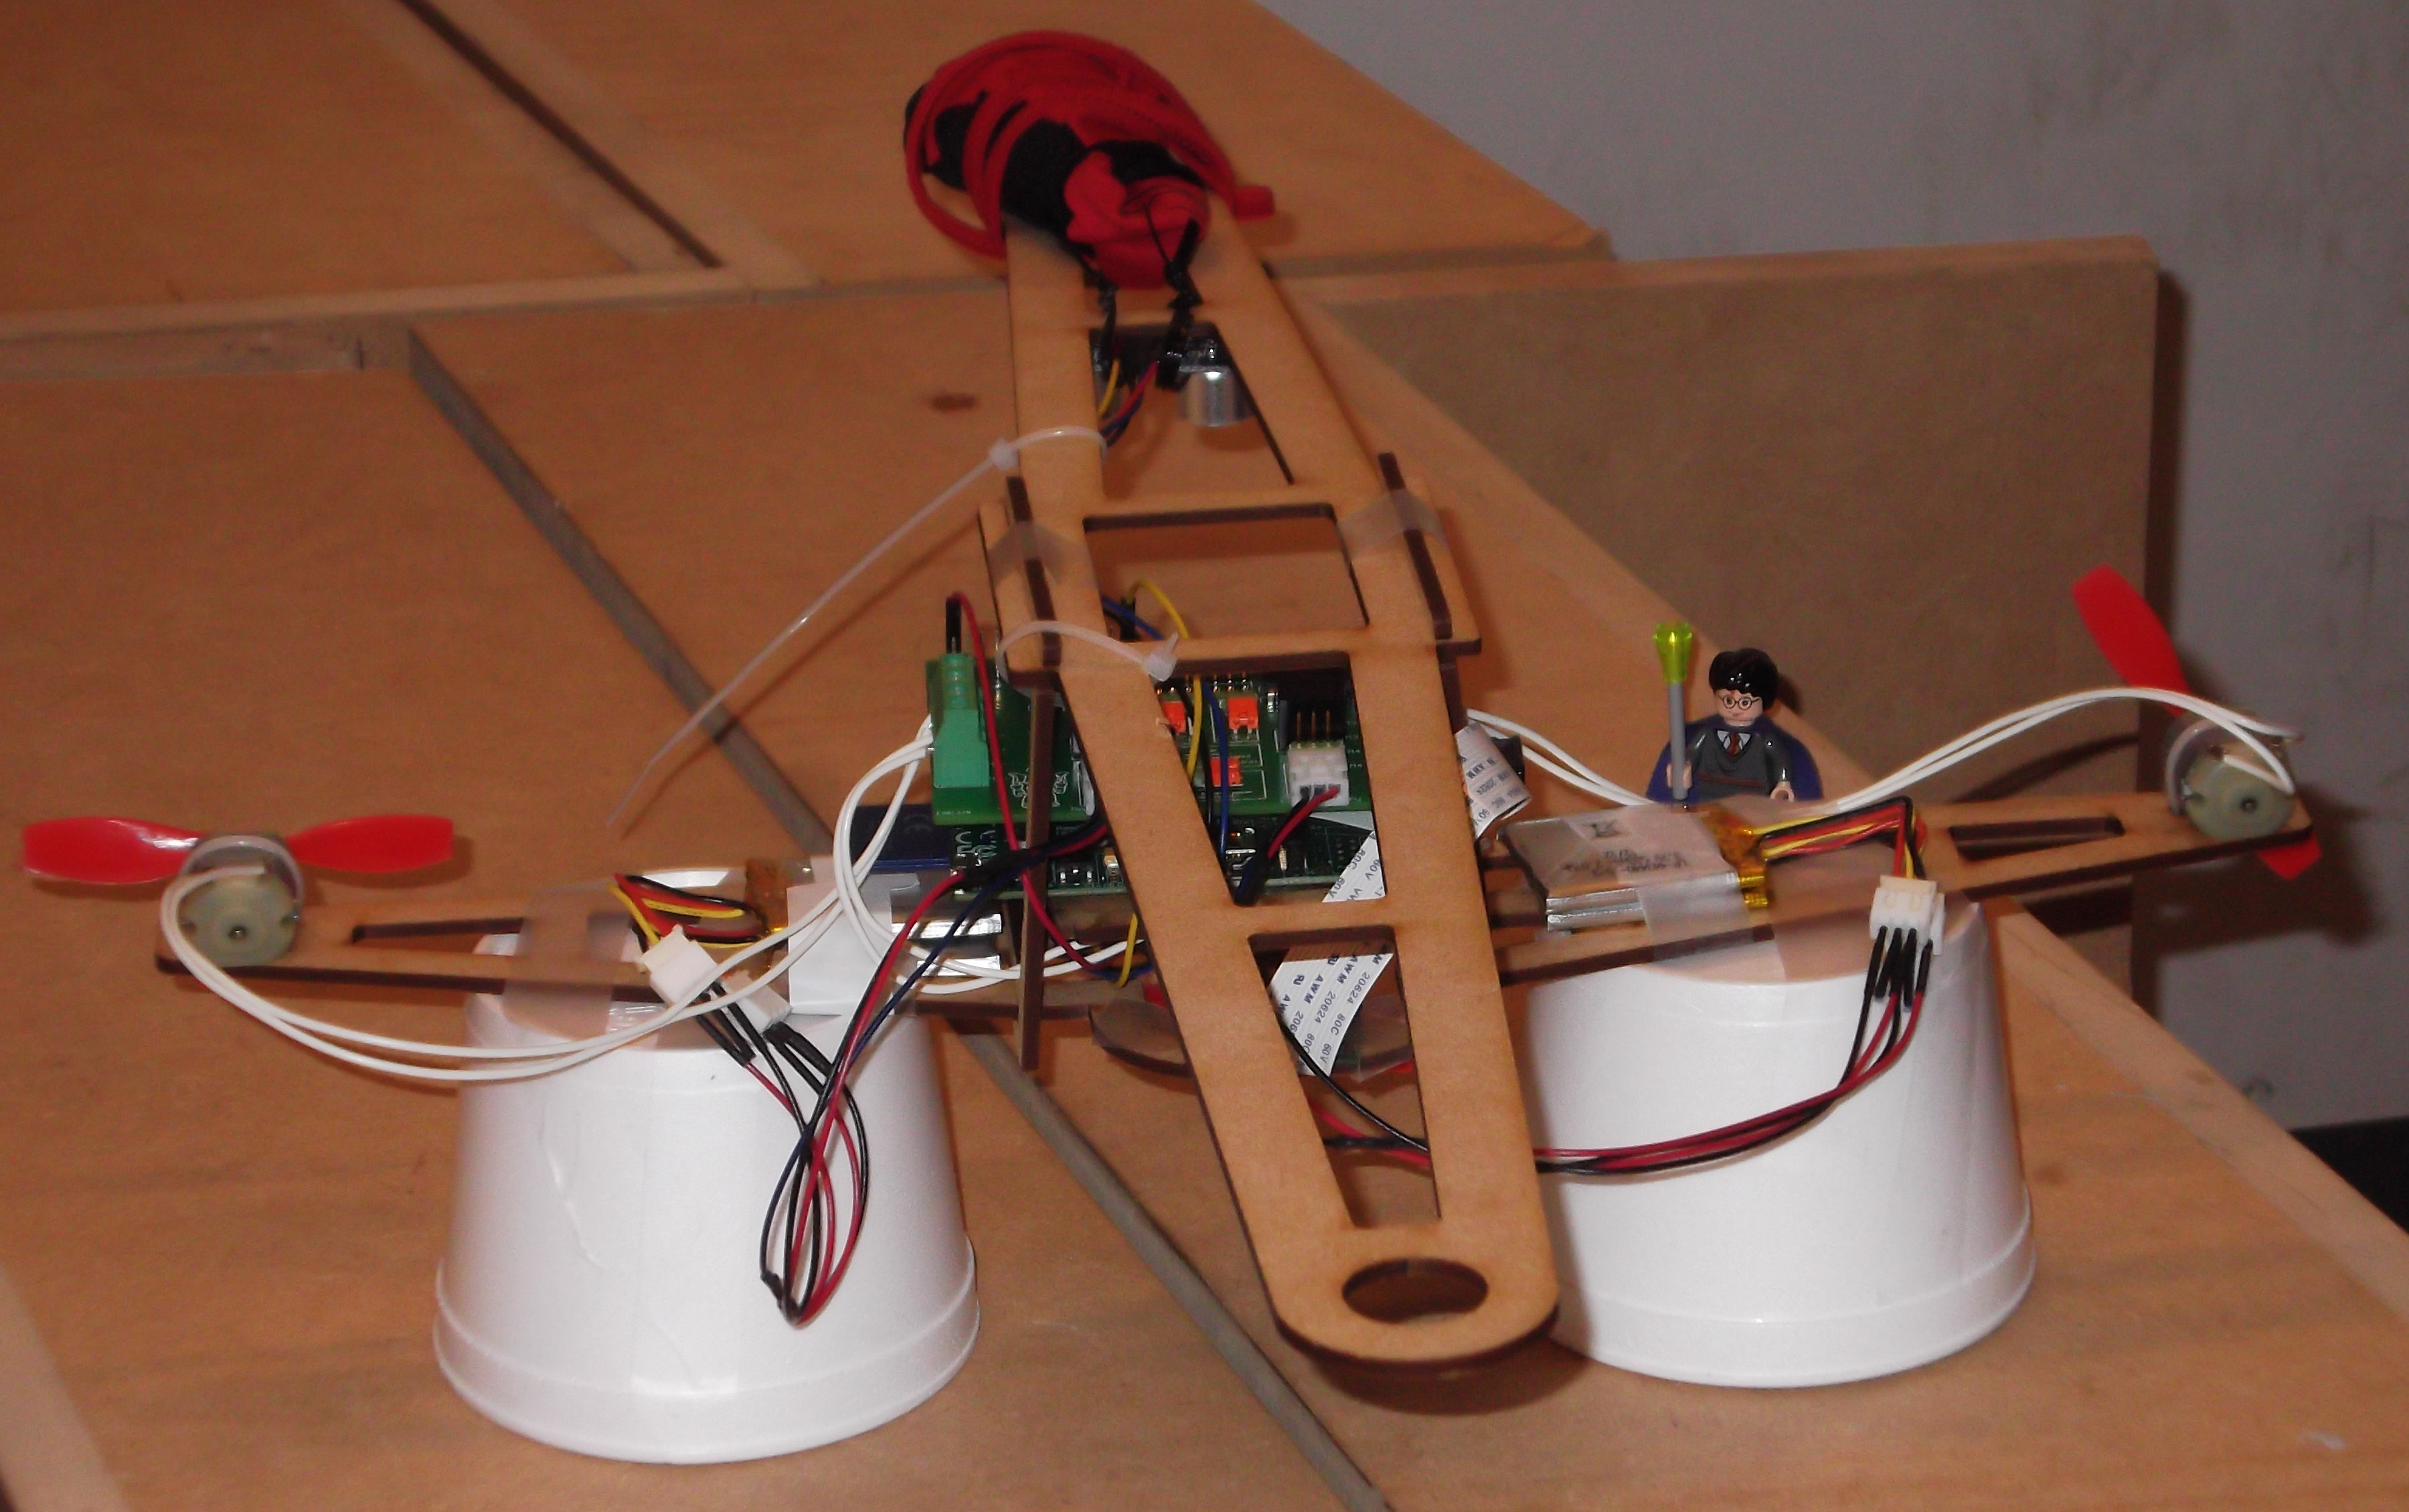
\includegraphics[height=60mm]{zeppelinFrame.jpg}
%\caption{Frame met gemonteerde onderdelen}
%\label{zeppFrame}
%\end{figure}

Om het geheel te monteren, hebben we gebruik gemaakt van plakband en zipties (bundelbandjes). We hebben bekertjes bevestigd om ballast te dragen, zodat het geheel lichtjes zakt wanneer de motor geen kracht naar boven zet. Als gewicht gebruiken we zout, zodat het mogelijk is om nauwkeurig het gewicht te regelen. Tijdens het landen steunt het geheel op twee pootjes, gemaakt van piepschuimen bekertjes. \\

% == Testen == %
\section{Testen}

Om er zeker van te kunnen zijn dat het aansturen van de zeppelin correct gebeurt, is het nodig dat de componenten getest worden. In deze sectie volgt hierover meer informatie.

\subsection{Afstandssensor}
Voor gedetailleerde gegevens verwijzen we naar het verslag onze zeppelin van het eerste semester (versie 2). Hier hadden we gemerkt dat een enkele waarde van de sensor niet noodzakelijk de correcte afstand weergeeft. Daarom houdt de afstandssensor de laatste 10 gemeten waardes bij. De huidige hoogte wordt gegeven als het gemiddelde van deze waardes (rolling median techniek). Het interval tussen twee metingen hebben we kunnen terugbrengen tot 20 ms.

\subsection{Camera en pattern recognition}
De implementatie van de pattern recognition vereist nieuwe testen van de camera om deze functionaliteit op punt te brengen. De tests proberen de verschillende moeilijkheden van de real time uitvoering te simuleren. De factoren die de positiebepaling aan de hand van de pattern recognition beinvloeden, betrekken zich grotendeels tot de lichtintensiteit, de hoogte en het nemen van foto’s terwijl de zeppelin beweegt. De verschillende factoren en hun bijbehorende tests worden hieronder besproken.\\
\textbf{Lichtintensiteit}\\
De intensiteit van het licht beinvloedt de detectie van de contouren en de kleuren. De belangrijkste fout bevindt zich bij de kleuren. Met behulp van een regelbare lichtbron en voldoende afschermeing van buitenaf neemt de camera foto’s van een patroon. Hierbij wordt de minimale benodigde lichtintensiteit geregistreert en dit wordt vergeleken met de lichtintensiteit aanwezig tijdens de uitvoering. \\
\textbf{Hoogte}\\
De hoogte van de zeppelin tijdens de fotoregistratie heeft gevolgen voor het aantal vormen die geregistreerd worden en de afstand tussen de vormen op de foto. Er is een minimaal aantal vormen nodig om de positie te bepalen (3 figuren). Indien er nog extra redundantie nodig is zodat indien een vorm de software een vorm niet herkent de plaatsbepaling toch succesvol is, zal er een minimale hoogte nodig zijn voor de zeppelin om foto’s te nemen. Het aantal pixels tussen de verschillende contouren kan ook een negatief effect hebben op de differentiatie van de verschillende vormen. De camera neemt foto’s van een patroon van vormen gepositioneerd onder de zeppelin waarbij de hoogte steeds varieert.\\ 
\textbf{Tijdens de beweging}\\
Als de zeppelin beweegt, kan dit effect hebben op de geregistreerde vormen. Een dilatie van de vormen kan plaatsvinden, waardoor een rechthoek zich tot een ruit omvormt bijvoorbeeld. Een ander mogelijk probleem constateert zich in het wazig worden van de foto’s waardoor image recognition niet met goede nauwkeurigheid plaatsvindt. Deze proef test het effect van de beweging  alsook de snelheid van de zeppelin op de dilatie van de figuren en de wazigheid van de foto’s.  \\


\subsection{Motoren}
In het eerste semester hebben we uitgebreide testen gedaan over de testen en de mogelijkheden van pwm. Het werd duidelijk dat het nodig ging zijn om constant de hoogte te controleren en bij te sturen. Daarnaast bleek ook dat horizontale bewegingen moeilijk exact kunnen worden uitgevoerd, omdat de zeppelin zeer gevoelig is voor allerlei veranderingen van de windomstandigheden in de omgeving: een andere zeppelin die beweegt, de airco, \ldots \\

In het tweede semester hebben we enkele nieuwe testen moeten uitvoeren, voornamelijk gerelateerd aan het gebruik van SoftPWM. Er moest bepaald worden tussen welke percentages het vermogen groot genoeg was om de motor effectief te laten draaien, net zoals we in het eerste semester hebben moeten doen. Dit gebeurde door middel van trial-and-error.  

% == ALGORITMES == %
\section{Algoritmes}
\subsection{Verticale bewegingen}
Om naar een bepaalde hoogte te stijgen, maken we gebruik van een PID-algoritme\footnote{http://www.csimn.com/CSI\_pages/PIDforDummies.html}. Hierbij gaan we op basis van de huidige fout in hoogte, bepalen of de zeppelin moet stijgen of dalen en met welke kracht. Daarnaast wordt rekening gehouden met de afgeleide, om toekomstige veranderingen te voorspellen. Tenslotte is er de integraal, die fouten uit het verleden voorstelt. Op basis hiervan wordt een pwm-waarde voor de motor gegeven. Het algoritme wordt aangepast aan het gewicht van onze zeppelin en de kracht van de gegeven motoren. \\
De output wordt berekend op basis van deze formule:

\begin{center}
\texttt{output = Kp*error + Ki*integral + Kd*derivative}\\
\end{center}

Hierin zijn Kp, Ki en Kd constanten die we hebben moeten bepalen. Eerst hadden we enkel rekening gehouden met de huidige error (Ki = Kd = 0), maar dit bleek er voor te zorgen dat de zeppelin veel te snel naar een bepaalde hoogte gaat en er dan ver boven of onder gaat. We hebben dit opgelost door Kd te verhogen. Door deze groot te maken, gaat de zeppelin veel rustiger naar de opgegeven hoogte en gaat hij er niet voorbij. Bij de start van het tweede semester hebben we de waardes van deze constanten opnieuw getuned, aangezien er nieuwe volle ballonnen gegeven waren. \\

Er is een HeightController die dit PID-algoritme implementeert, en die er voor gaat zorgen dat de zeppelin zijn hoogte behoudt of naar een gevraagde hoogte gaat. Deze gaat om de 0.1 s de hoogte controleren en de pwm-waarde bijsturen. \\

\subsection{Horizontale bewegingen}
Voor bewegingen in het horizontale vlak maken we eveneens gebruik van een PID-gebaseerd algoritme. Hiervoor zijn er twee afzonderlijke algoritmes die tegelijk lopen (voor de x- en y-richting). Er wordt gebruik gemaakt van de huidige positie van de zeppelin, de co\"{o}rdinaten van de bestemming, en de rotatie van de zeppelin. De positie en rotatie zijn af te leiden van de gegevens die de camera doorstuurt. De verwerking van die gegevens leidt tot de benodigde co\"{o}rdinaten.

\subsection{Pattern recognition}
De camera neemt foto’s van de patronen op het veld onder de zeppelin. De Raspberry Pi bewerkt deze foto’s met behulp van zelfgeschreven software. Op elk geregistreerd beeld worden dezelfde sequentie van operaties uitgevoerd. 
Als eerste herkent de software de simpele vormen. De functionaliteit van het programma beperkt zich tot de mogelijke vormen meegedeeld in de probleemstelling (cirkel, rechthoek, vijfpuntige ster, hart, ruit). De vormherkenningalgoritmes (pattern recognition) registreren de contouren van deze vormen en halen de nuttige contouren uit het waargenomen beeld. De contourbenadering kan contouren herkennen die niet bij de vormen horen en dus onnuttig zijn en verwijderd worden. Vervolgens benadert de software de overgebleven contouren door polygonen (veelhoeken). Op basis van de punten van deze benaderingen en kenmerken van de mogelijke vormen haalt het algoritme de corresponderende vorm(en) uit de foto. Bijvoorbeeld: De punten op een cirkel bevinden zich op een vaste afstand van het middelpunt, de lengte van een rechthoek is gelijk aan de gesommeerde afstand tussen de de vier hoekpunten... 
Eenmaal de vorm gespecificieerd is, dient de kleur nog bepaald te worden.  Het programma converteert hiervoor de foto naar een HSV-digitale voorstelling. De minimale en maximale waarden voor respectievelijk H,S en V, die karakteristiek zijn voor de mogelijke kleuren, bepalen de aanwezige kleur binnen de contour van de aanwezige vorm. 


% == SOFTWARE == %
\section{Software}

Alle software voor dit project is in Java geschreven. Dit is gekozen omdat dit voor het hele team de meest gebruikte programmeertaal was. Dit gaf wel een verschillende moeilijkheden bij het implementeren van een aantal aspecten (image recognition, \ldots). \\

\begin{figure}[H]
\begin{center}
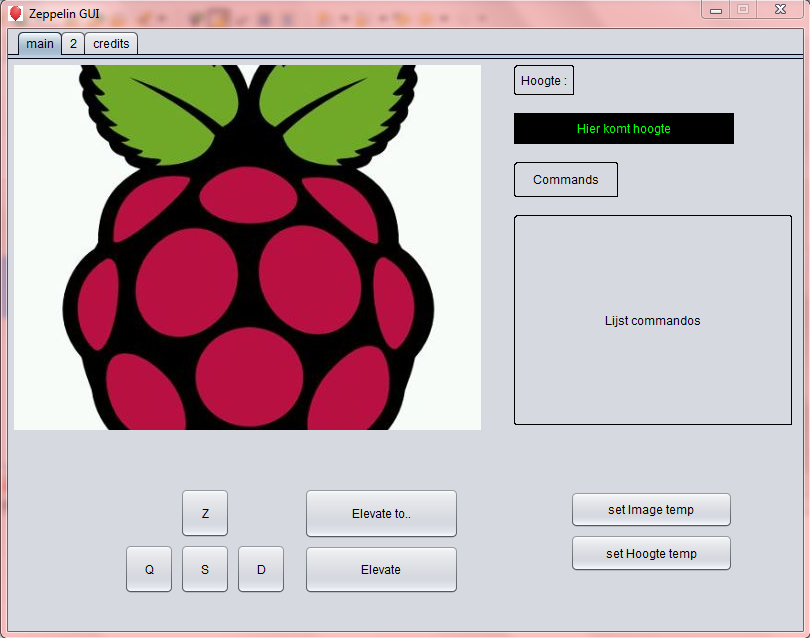
\includegraphics[width=0.45\textwidth]{GUI.png}
\end{center}
\caption{GUI}
\label{GUI}
\end{figure}

\textbf{GUI} \\
De Graphical User Interface stelt de gebruiker in staat om vanaf een client-pc verbinding te maken met de server die het speelveld en de zeppelins controleert. De GUI geeft dan informatie weer over het speelveld en de co\"{o}rdinaten van de zeppelins.  \\

De eerste tab (`overview') toont de hoogte van beide zeppelins, alsook de toestand van de eigen propellers. Een kaart geeft de locaties van de zeppelins weer. Voor het maken van deze kaart wordt gebruik gemaakt van een CSV-bestand(comma separated value). Hierin wordt elk roosterpunt voorgesteld door twee letters: een voor de kleur en een voor de vorm van de figuur op dat punt. Naast de kaart wordt de opdracht van de zeppelins getoond en is er een overzicht van de laatste berichten die zijn uitgewisseld tussen de client-pc en de zeppelin. \\

De tweede tab geeft een uitgebreider overzicht van alle informatie die wordt uitgewisseld tussen de GUI en zeppelin, met een indicatie van de tijd. Er is een mogelijkheid om berichten te filteren op type. \\



\textbf{Pattern recognition}\\
De eerder vermelde pattern recognition is gemaakt met behulp van de Java-library OpenCV\footnote{http://opencv.org/}. Hiermee kan detectie van vormen en kleuren worden ge\"{i}mplementeerd. \\

\textbf{Connectie}\\
De verbinding tussen Pi en laptop is volledig veranderd. Voordien werd informatie uitgewisseld door middel van sockets, waar de client(laptop) op poort 6789 connecteerde. De Pi fungeerde dan als server omdat deze de sockets initialiseerde. Deze opdracht verplicht ons gebruik te maken van een RabbitMQ server\footnote{www.rabbitmq.com}. Voor de eerste tussentijdse demo zal de server op één van onze eigen laptops worden gestart, omdat er geen communicatie met een andere zeppelin nodig is. De laptop is nu de server en de Pi is client. Zowel laptop als Pi connecteren dan op een exchange genaamd ‘server’. Elke boodschap dat wordt uitgewisseld krijgt een bepaalde sleutel toegewezen. een boodschap wordt dan naar de exchange verstuurd. De exchange weet dankzij de sleutel naar welke queue hij de boodschappen moet versturen.  Zowel de laptop als de Pi abonneren zich op queues met een bepaalde sleutel, afhangende van welke gesleutelde boodschappen ze willen ontvangen. Om gebruik te maken van rabbitmq in onze code moesten er welke enkele libraries\footnote{http://www.rabbitmq.com/java-client.html} toegevoegd worden. Voor een sequentiediagram van de communicatie, zie bijgevoegde figuur.
\\

\begin{figure}[H]
\begin{center}
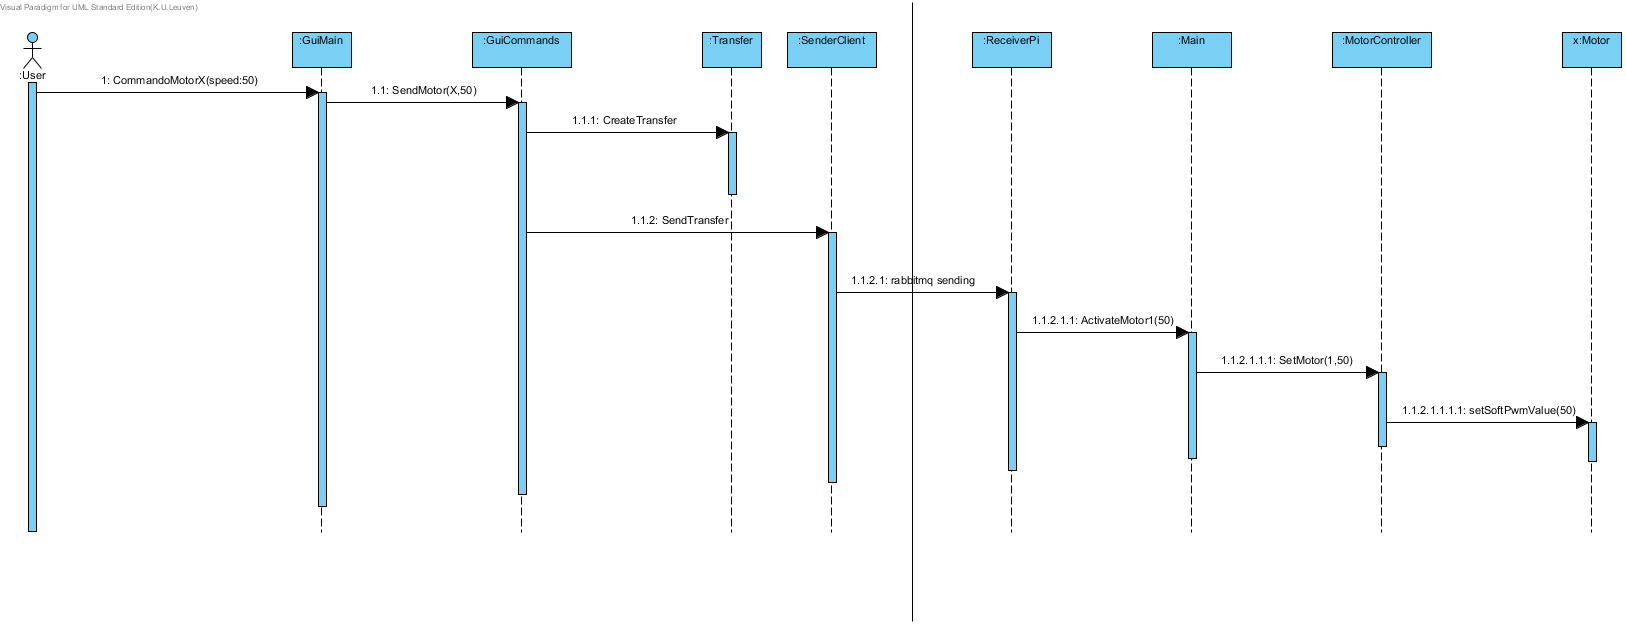
\includegraphics[width=1\textwidth]{PiToClientCommunication.png}
\end{center}
\caption{Sequentiediagram van de communicatie}
\label{Sequence}
\end{figure}






% == BESLUIT == %
\section{Besluit}
De uitvoering van de toevoegingen aan soft- en hardware zijn vrij goed gelukt. Het implementeren van pattern recognition en de bijhorende navigatie bracht wel enkele moeilijkheden met zich mee. Na veel nattevingerwerk is het gelukt om dit helemaal werkend te krijgen. Het communiceren met een RabbitMQ-server hadden we vrij snel onder de knie en was dus snel ge\"{i}mplementeerd. De GUI slaagt erin om een ingelezen map duidelijk weer te geven, en de positie van de eigen zeppelin kan getekend worden. 

Tegen de volgende deadline moeten we meer vliegtesten uitvoeren. Ook moeten we de zeppelin in contact brengen met een andere zeppelin. Hij moet hiermee draadloos kunnen communiceren via de server. Ook moeten de zeppelins er zelf voor zorgen dat ze niet botsen. Hiervoor moet er nog software geschreven worden. 


% == APPENDICES == %
\newpage\makeappendix

\section{Beschrijving van het proces}
Dit onderdeel maakt geen deel uit van dit verslag.


\section{Beschrijving van de werkverdeling}

Hieronder is een tabel te vinden met de gewerkte uren binnen en buiten de sessies: \\

\begin{tabular}{r||r|r|r|r|r}
Overzicht: & Dimitri Jonckers & Wander Bavin & Wout Vekemans & Sunil Tandan & Vince Goossens \\
\hline \hline
09/02 - 15/02 &  &  &  &  &  \\
\hline \hline
Totaal &  &  &  &  &  \\
\end{tabular}


\section{Kritische analyse}
Dit onderdeel maakt geen deel uit van dit verslag.


\end{document}
